\chapter{Related Work} % (fold) ===============================================
\label{cha:background}
Bipedal locomotion is one of the most active areas of research within humanoid robotics. This section presents a brief literature review on the design and gait synthesis for humanoid robotic applications. 



%==============================================================================
%   E L E C T R O M E C H A N I C A L   D E S I G N 
%==============================================================================



\section{Humanoid Electromechanical Design} % (fold) ==========================
\label{sec:related_electromechanical_design}
The electromechanical design of humanoid robots have undergone several generations of revisions. 


\subsection{Degrees of Freedom} % (fold) ======================================
\label{sub:related_degrees_of_freedom}
The selection of degrees-of-freedom (DOF) of a humanoid robot plays an essential role in the design and development phase. 
% subsection degrees_of_freedom (end) =========================================


\subsection{Mechanism Design} % (fold) ========================================
\label{sub:related_mechanism_design}
Linkage subsystems used to carry out motion is also an area where several approaches exist. 
% subsection mechanism_design (end) ===========================================


\subsection{Passivity-Based Designs} % (fold) =================================
\label{sub:related_passive_designs}
Perhaps the simplist approach to designing bipedal robots are those without any active power. 
% subsection passivity_based_designs (end) ====================================


\subsection{Actively-Powered Designs} % (fold) ================================
\label{sub:related_active_designs}
The most common approach to electromechanical design for bipedal robots is through the generation of active power for locomotion. 
% subsection actively_powered_designs (end) ===================================


% section humanoid_electromechanical_design (end) =============================



%======================================================================
%   W A L K I N G  C O N T R O L  &  G A I T  G E N E R A T I O N
%======================================================================



\section{Walking Control Strategies and Gait Generation} % (fold) =============
\label{sec:related_control_strategies}
There exists a wide range of control strategies to achieve bipedal locomotion in robotics literature to date. Some of the most popular strategies are briefly reviewed in this section.


\subsection{Zero-Moment Point} % (fold) =======================================
\label{sub:related_zero_moment_point}
The most popular techniques to achieve walking have been trajectory generation and control strategies based on the Zero-Moment Point (ZMP) criterion \cite{Vukobratovic:2004wy}. The ZMP defines a point on the ground where the forces acting on a biped do not produce a moment about the axes parallel to the ground plane. If the ZMP is kept within the region of foot support, the biped is stable. This stability criterion can be used to compute ZMP-stable trajectories offline that maximize the stability margin by maximizing the distance from the ZMP to the boundary of the support region. In the on-line phase, the stable trajectories are tracked online to execute walking \cite{HuangEtAlTRA2001}.  ZMP-based trajectories can also be generated on-line \cite{KajitaEtAlICRA2003,TakenakaEtAlIROS2009}. 

One of the biggest drawbacks of this approach is the resulting trajectory does not provide any strategy to respond to disturbances due to uneven terrain or unexpected forces. Typically, these strategies \cite{Kajita:1997vr,Kajita:2001fk,Sugihara:2002kq} are also energetically inefficient since they are constantly trying to maintain balance by keeping the ZMP point within the region of foot support. Furthermore, the resulting gait does not utilize the natural dynamics of the system and consequently does not look human-like. Despite the drawbacks, some of the most popular humanoid robots today utilize some variation of ZMP based feedback for bipedal locomotion. The most popular application is the famous Honda Asimo \cite{Hirai1998}. Newer bipeds available for research like Aldebaraan's Nao \cite{Gouaillier2006} robot also use ZMP-based walking control strategies. 
% subsection zero_moment_point (end) ==========================================


\subsection{Passive Dynamics} % (fold) ========================================
\label{sub:related_passive_dynamics}
An alternative approach, first proposed by McGeer \cite{McGeer:1990uk}, introduced a unique class of legged robots known as passive dynamic walkers \cite{Collins:2005vp}. This approach takes advantage of the natural dynamics of the biped structure, and is capable of maintaining a stable gait cycle without active control effort. Fully passive mechanisms walk on an inclined surface so that the mechanism is powered by gravity alone \cite{Spong:1999vk}. In addition to producing highly efficient walk, the gait patterns generated using this approach appear more human-like in comparison to ZMP-based control. However, passive dynamic walkers lack robustness to perturbations due to very narrow regions of attraction.

Thus far, majority of the research in passive dynamics has been restricted the very specific scenario of walking on an incline. This lacks the versatility that is required for humanoid robots if they are to ultimately navigate in most human environments (level ground). Further investigative research was helpful in characterizing the nature of a passive gait cycle \cite{Goswami:1996gn} in terms of stability and energies. This ultimately gave rise to new strategies which were aimed towards emulating the work done by gravity on an inclined slope \cite{Asano:2000wi}. These hybrid approaches known as virtual passive dynamics improved the versatility of the simple legged robots to walk on level ground with minimal actuation as a replacement for gravity \cite{Asano:2004tv}. 

While these minimally actuated bipeds have been shown to exhibit similar energetics as purely passive machines \cite{Asano:2004jp}, most research is typically restricted to 2D dynamics in the sagittal plane. The challenges of extending these simple models to 3D (i.e. incorporating lateral dynamics) lies in the unstable motion introduced by mismatch of roll velocity and contact conditions \cite{Kuo:1999tn}. This is particularly challenging since even small disturbances can be completely destabalizing for passive dynamic walkers. Although the minimal actuation strategy based on passive dynamics is more versatile, the main difference between the two approaches simply boils down the source of energy used for walking. Regardless of the source, the quantity of energy provided stay within a stable limit cycle depends only on the slope of the incline \cite{Goswami:1996gn}. Thus, stabilizing the dynamics in both sagittal and frontal planes is particularly challenging since both strategies share the same underlying weakness to perturbations. 
% subsection passive_dynamics (end) ===========================================


\subsection{Force/Impedance} % (fold) =========================================
\label{sub:related_force_impedance}
\Incomplete
% subsection force_impedance_control (end) ====================================


\subsection{Machine Learning} % (fold) ========================================
\label{sub:related_machine_learning}
\Incomplete
% subsection machine_learning_strategies (end) ================================


\subsection{Foot Placement} % (fold) ==========================================
\label{sub:related_foot_placement}
Recently, an alternative problem formulation focusing on restoring balance has been proposed. The Foot Placement Estimator (FPE), introduced by Dwight et al \cite{Wight:2008ii} formulates an approach to restore balance by controlling swing foot position during the gait cycle. By using the conservation of angular momentum, the FPE equation determines the location on the ground where the total energy of an unstable biped after swing foot impact is equal to the peak potential energy. If a step is taken before the FPE location, the post impact energy of the system causes the biped to fall over. Conversely, stepping beyond the FPE location on the ground causes the biped to fall back onto the hind leg.

The solution to the FPE equation itself can be used as a recovery mechanism (i.e. in the face of a destabilizing disturbance) with existing ZMP-based strategies. Alternatively, it can be used to increase the narrow regions of attraction which plague minimally actuated passive dynamic walkers \cite{Goswami:1996gn,Asano:2000wi,Kuo:1999tn}. The key concept here is that the FPE-based integration would require minimal joint actuation only to align a swing food appropriately to recover from a potential fall. As shown in \cite{Wight:2008ii,Wight:2008vt}, FPE can also be extended to form complete gait cycles to achieve dynamically stable walking. However, there are several key assumptions which are violated when attempting to implement this approach on a physical 3D robot. Namely, the theory presented in the derivations assume that the legs are massless and it only deals with the 2D dynamics in the sagittal plane.

The capture point concept, developed by Pratt et al. \cite{Pratt:2006vy}, is conceptually similar to the FPE. While the derivation of FPE is based on a simple compass biped model with fixed parameters, the capture point theory was derived using complex motion models which included using a flywheel body to control/offset any disturbances through the use of rotational inertia. Ultimately, the simplicity of the model allowed the FPE theory to be extended to complete gait cycles, while the work presented by Pratt et al simply solved the problem of lateral stabilization \cite{Wight:2008ii}.

Recently, a more comprehensive approach using the capture point for foot placement as a means to develop full walking control strategies has been proposed. De Boer \cite{DeBoer:2012wp} focused on the ground/foot interaction to develop a robust and energetically efficient walking control strategy for a force-controlled compliant lower-body biped. While this approach is philosophically similar to the idea behind FPE, there are several key differences. The approach presented in this thesis uses simple local controllers to form complete gait cycles and can be used on position-controlled joints without any complex actuation systems. The capturability framework demonstrated in \cite{Pratt01092012} used separate controllers for the swing and stance legs whereas this approach uses a single global differential kinematic resolution for whole body motion control.
% subsection foot_placement_strategies (end) ==================================


% section walking_control_strategies_&_gait_generation (end) ==================



%======================================================================
%   2 D  F O O T  P L A C E M E N T  E S T I M A T O R
%======================================================================



\section{FPE Algorithm in 2D} % (fold)
\label{sec:fpe_algorithm}
The existing 2D FPE theory introduced in Section~\ref{sub:related_foot_placement} is briefly reviewed in this section. The significance of the FPE point on the ground is demonstrated through simulation. 

Consider the standard compass biped model used widely in bipedal locomotion research today (shown in Figure \ref{fig:compass}). This simplified model is commonly used as the first step to reduce the complex dynamics to the two dimensional sagittal plane. The physical parameters are the mass $m$, inertia about the center of mass $I_{COM}$, leg lengths $L$ and leg separation angle $\beta$. Note that the angle $\theta_A$ is measured from the axis normal to the ground. 

\begin{figure}[!h]
	\centering
    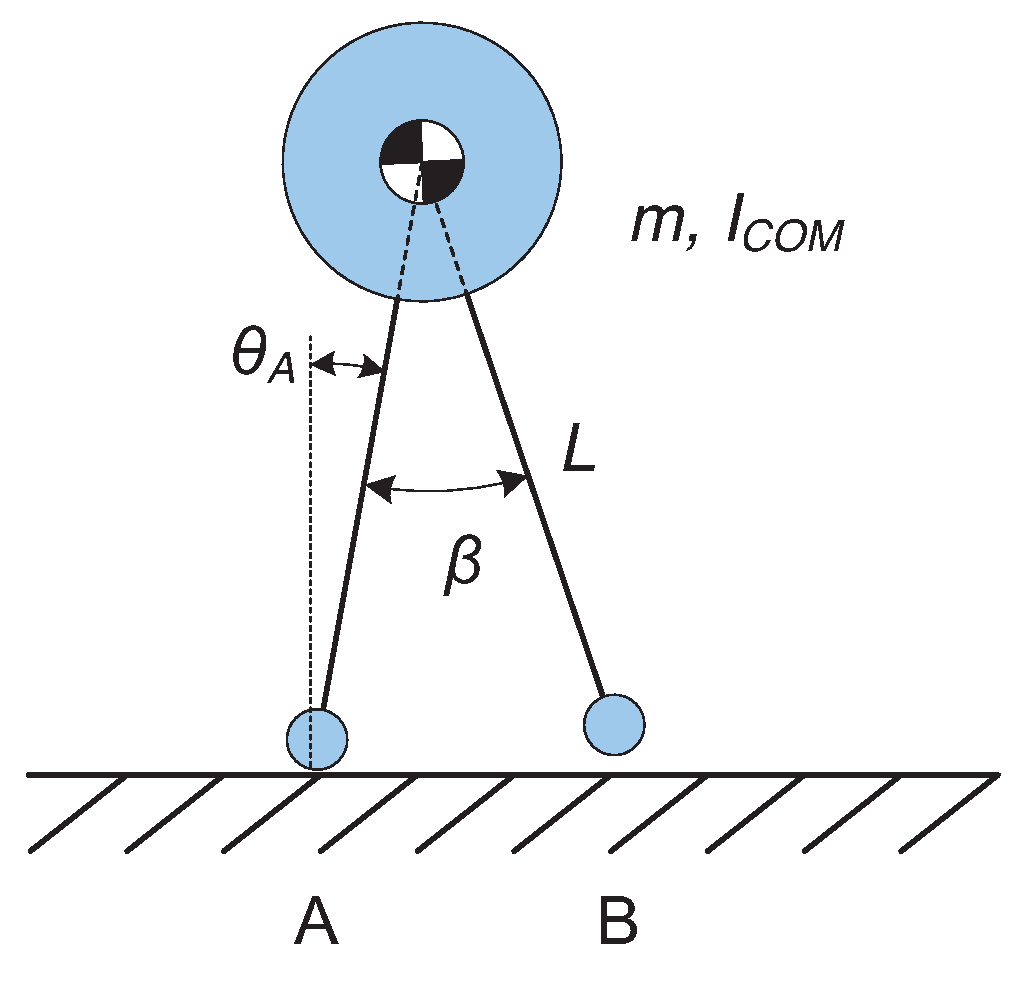
\includegraphics[scale=0.4]{fig/fpe/fig1.eps}
  	\caption{Standard compass biped model used for nonlinear analysis  and derivation of the FPE equation.}
	\label{fig:compass}
\end{figure}

Now consider this system at the moment when the swing leg comes into contact with the ground at point $B$ (the resulting behaviour is illustrated in Figure \ref{fig:prepost}). The following assumptions are made in reference to the behaviour of the system around the pre-impact and post-impact stages to simplify the model for further analysis \cite{Wight:2008vt}: 

\hrulefill

\begin{assumption}
	There is an instantaneous transfer of balance (i.e. the stance foot at point $A$ lifts up when the swing foot hits the ground at point $B$).  
\end{assumption}

\begin{assumption}
	The impact when the swing leg hits the ground at point $B$ is assumed to plastic. 
\end{assumption}

\begin{assumption}
	There is sufficient friction to prevent any slipping at the contact points. 
\end{assumption}

\begin{assumption}
	Gravity is assumed to be a non-impulsive force. 
\end{assumption}

\begin{assumption} \label{assump:betafix}
	The leg separation angle $\beta$ is fixed.
\end{assumption}

\begin{assumption} \label{assump:massless}
	The legs are massless and therefore do not significantly alter the dynamics of the system. 
\end{assumption}

\hrulefill

Note that assumption \ref{assump:betafix} implies that if both feet were to remain on the ground (i.e. double support phase), then by geometric symmetry about the normal, $\theta _A = \beta/2$. Equivalently, when leg $A$ is completely vertical, $\theta _A = 0$.

\begin{figure}[!h]
	\centering
    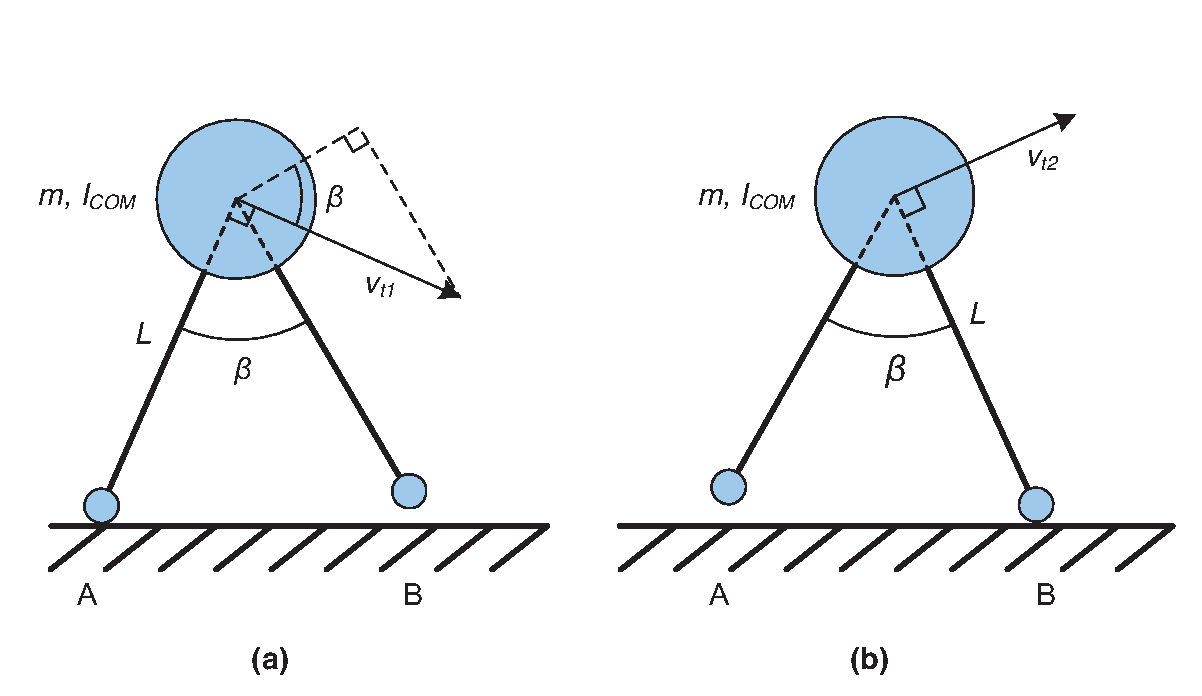
\includegraphics[scale=0.6]{fig/fpe/fig2.eps}
  	\caption{Compass biped model in the swing phase of the gait cycle in the (a) pre-impact and (b) post-impact configurations.}
	\label{fig:prepost}
\end{figure}

\subsection{Equations of Motion}

To formulate a state space representation of the biped, the equations of motion are derived as follows\footnote{Only key points of the derivation are summarized, for details on the full derivation of the FPE equation can be found in \cite{Wight:2008vt,Millard:2011vk}}. If the biped is treated as an inverted pendulum rotating about pivot point $A$ (i.e. configuration shown in Figure  \ref{fig:compass}), the equation of motion is found by applying Newton's second law:

\begin{equation}
	\begin{aligned}
		\sum {{\tau _A} = {I_A}} {{\ddot \theta }_A}
	\end{aligned}
\end{equation}

\begin{equation} \label{eq:compasseom1}
	\begin{aligned}
		{{\ddot \theta }_A} = \frac{{mgL\sin ({\theta _A})}}{{{I_{COM}} + m{L^2}}}
	\end{aligned}
\end{equation}

This equation is only valid while the inverted pendulum swings about point $A$ (i.e. pre-impact). When the swing leg comes in contact with the ground and based on the assumptions, point $B$ becomes the new pivot for inverted pendulum (post-impact). The motion of the post-impact system is now based on a different angular velocity (namely, $\dot{\theta}_B$). However, the assumptions 1-4 also relate the angular momentum of the system in the pre-impact stage (Figure \ref{fig:prepost}a) to the post-impact stage (Figure \ref{fig:prepost}b). Applying the conservation of angular momentum about point $B$, the post-impact angular velocity ($\dot{\theta}_B$) is a function of the pre-impact angular velocity ($\dot{\theta}_A$) \cite{Wight:2008vt} by the following: 

\begin{equation}
	\begin{aligned}
		{\dot \theta _B} = \frac{{({L^2}m\cos (\beta ) + {I_{COM}}){{\dot \theta }_A}}}{{{L^2}m + {I_{COM}}}}
	\end{aligned}
\end{equation}

While pivoting about point $B$, if the biped does not have enough momentum to swing all the way through then it simply rocks back until swing leg $A$ comes into contact with the ground. At this point, the equation of motion describing the system reverts back to \eqref{eq:compasseom1}. Given the geometric properties of the biped, it can be shown that the equation of motion about point $B$ is given by: 

\begin{equation} \label{eq:compasseom2}
	\begin{aligned}
		{\ddot \theta _B} = \frac{{mgL\sin ({\theta _B})}}{{{I_{COM}} + m{L^2}}} 
	\end{aligned}
\end{equation}

Together, $\theta _A$, $\theta _B$, along with its derivatives completely describe the motion of the compass biped. 

\subsection{Unified State Equations}
Assumption 5 imposes a geometric constraint which can be used to combine the variables which completely define the motion. At the instant of impact, the angles $\theta _A$ and $\theta _B$ can be expressed as: 

\begin{equation}
	\begin{aligned}
		{\theta _A} = \theta  + \frac{\beta}{2} \\
		{\theta _B} = \theta  - \frac{\beta}{2}
	\end{aligned}
\end{equation}

Where the angles $\theta _A$, $\theta _B$, $\theta$ and $\beta$ are shown on Figure \ref{fig:unified}. The single (unified) variable $\theta$ can be formed by rearranging the equations of motion described in terms of $\theta _A$ and $\theta _B$: 

\begin{subnumcases}{\ddot{\theta}=\label{eq:unifiedeom}}
	\frac{{mgL\sin (\theta  + \beta /2)}}{{{I_{COM}} + m{L^2}}} & $\theta < 0$ \\
	\frac{{mgL\sin (\theta  - \beta /2)}}{{{I_{COM}} + m{L^2}}} & $\theta > 0$ \\
	\frac{{mgL\sin (\theta  + \beta /2)}}{{{I_{COM}} + m{L^2}}} & $\theta = 0$, $\dot{\theta} > 0$ \\
	\frac{{mgL\sin (\theta  - \beta /2)}}{{{I_{COM}} + m{L^2}}} & $\theta = 0$, $\dot{\theta} < 0$ \\
	\quad \quad \quad \quad 0 & $\theta = 0$, $\dot{\theta} = 0$
\end{subnumcases}

The system defined by \eqref{eq:unifiedeom} is used to investigate stability and subsequently derive the FPE equation. For future reference, define the following function to represent conditional equation of motion corresponding to a region of the state space (defined by $\theta$ and $\dot{\theta}$): 

\begin{equation}  
	\begin{aligned}
		\ddot{\theta} \eqdef F(\theta, \dot{\theta})
	\end{aligned}
\end{equation}

\begin{figure}[!t]
	\centering
    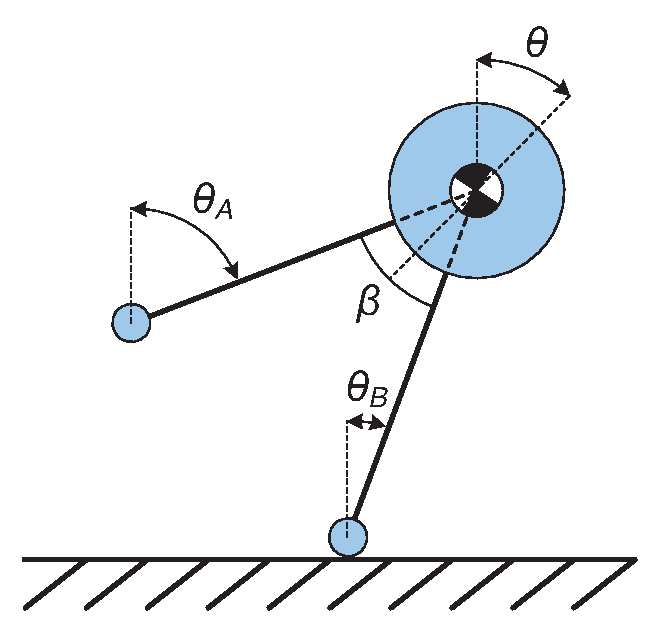
\includegraphics[scale=0.7]{fig/fpe/fig3.eps} 
  	\caption{Unified variable $\theta$ used to simplify the analysis. It is easily observed that $\theta_A = \theta  + \beta /2$ and $\theta_B = \theta  - \beta /2$}.
	\label{fig:unified}
\end{figure}

This unified variable is used to form a state space representation with the states as $\theta$ and $\dot{\theta}$: 

\begin{equation} \label{ss}
	\begin{aligned}
				\begin{gathered}
  			\dot{\Theta} = \left[ {\begin{array}{*{20}{c}}
  {\dot \theta } \\ 
  {F(\theta, \dot{\theta})} 
							   \end{array}} \right]
		\end{gathered}
	\end{aligned}
\end{equation}

\subsection{Conditions for Stability}
The notion of stability (or lack there of) is explicitly defined by \cite{Wight:2008vt} as follows: 

\hrulefill

\begin{definition} \label{def:fallen}
	The biped has fallen if $\dot{\theta} = 0$ and any other point other than the feet is in contact with the ground. 
\end{definition}

\begin{definition} \label{def:balanced}
	The biped is balanced if $\dot{\theta} = 0$ and it has not fallen. 
\end{definition}

\begin{definition} \label{def:stable}
	The biped has stable if for a given set of initial conditions and no further energy input to the system, the biped eventually comes to a rest in an upright position. Once at rest, a sufficiently small, impulsive, nonzero external disturbance to the biped should result in motion that will eventually return to the same stable, balanced position. 
\end{definition}

\hrulefill

\begin{figure*}[!t]
	\begin{equation} \label{eq:fpe}
	\begin{aligned}
		\frac{{{{\left[ {mh({v_x}\cos \phi  + {v_y}\sin \phi )\cos \phi  + {I_{COM}}{{\dot \theta }_1}{{\cos }^2}\phi } \right]}^2}}}{{m{h^2} + {I_{COM}}{{\cos }^2}\phi }} + 2mgh\cos \phi (\cos \phi  - 1) = 0
	\end{aligned}
	\end{equation}
	\\ 
	\hrulefill
\end{figure*}

The only physical configuration that can be achieved by definition \ref{def:balanced} is if the biped is double support phase. This implies that being balanced is mathematically equivalent to the system $\dot{\Theta}$ remaining at its stable equilibrium at the origin. The second part of definition \ref{def:stable} implies that stability in the physical sense is equivalent to the origin of system $\dot{\Theta}$ being asymptotically stable (since the biped should return to the same balanced position after small enough perturbations.

Thus, it is possible to determine the conditions for which the biped is stable if it it can be shown that the origin of \eqref{ss} is asymptotically stable. To this end, a Lyapunov function candidate based on the energy of the system ($U = T + V$) with an offset in potential energy is chosen to show asymptotic stability. For example, for the first equation of motion represented by \eqref{eq:unifiedeom} for $\theta < 0$: 

\begin{equation}
	\begin{aligned}
		V(\Theta) &= {\frac{1}{2}({I_{COM}} + m{L^2}){\dot \theta ^2} + mg(h - {h_{datum}})}	
		\end{aligned}
\end{equation}

Where $h =\cos (\theta+\beta/2) $ and $h_{datum} = \cos (\beta/2)$. The Lyapunov candidate is positive definite if $-\beta/2 < \theta < \beta/2$ with the following $\dot{V}(\Theta)$: 

\begin{equation}
	\begin{aligned}
			\dot{V}(\Theta) &= ({I_{COM}} + m{L^2}){\dot \theta ^2}F(\theta ,\dot \theta ) - mgL\sin (\theta  + \beta /2)\dot \theta
	\end{aligned}
\end{equation}

Analyzing the behaviour of $\dot{V}(\Theta)$ involves looking at each region of the state space specified by \eqref{eq:unifiedeom} and investigating the behaviour within the local region. In summary, $\dot{V}(\Theta) = 0$ for the cases where $\theta \not= 0$  (i.e. \ref{eq:unifiedeom}a and \ref{eq:unifiedeom}b) and is negative definite when $\theta = 0$, $\dot{\theta} \not= 0$ (i.e. \ref{eq:unifiedeom}c and \ref{eq:unifiedeom}d). Furthermore, the equilibrium point is the largest invariant set in: 
\[E = \left\{ {\Theta |\dot V(\Theta ) = 0} \right\}\]
Thus, by the Barbashin-Krasovskii-LaSalle principle it is shown that origin of $\dot{\Theta}$ is locally asymptotically stable in the sense of Lyapunov. In order to determine which initial conditions will exhibit a decaying orbit towards the origin, the exact boundaries of the local stability is obtained by analyzing the behaviour of the total system energy with different initial conditions. 

\subsection{Computing the FPE Angle} % (fold)
\label{sub:computing_the_fpe_angle}
Given that the system is asymptotically stable and the exact boundaries of the local stability are defined, it is possible to determine whether a specific location in the state space is stable in the sense of definition \ref{def:stable}. However, the goal for FPE is to determine where the foot must be placed in order to restore stability, so the knowledge of the local stability is used to reformulate the problem. 

To this end, the approach described in \cite{Wight:2008vt} introduces a parameter known as the FPE angle ($\phi$). The projection from the COM at an this angle $\phi$ to the ground surface provides the location of where the foot would need to be placed in order to restore stability to the unbalanced system. The actual solution to \eqref{eq:fpe} yields the FPE angle $\phi$, which can be obtained by using numerical techniques for solving non-linear equations. In essence, the FPE angle $\phi$ specifies the configuration system to enter/remain inside the locally stable region of $\dot{\Theta}$ if it were to step in the \textit{next} instant. By continuously tracking this angle while the biped is about to land the swing foot, the angle $\phi$ eventually converges to $\beta/2$ prior to impact.

Note that so far, the simple compass biped model used made several assumptions which are now lifted. The leg separation angle $\beta$ is no longer a fixed value throughout the whole gait cycle. Instead, by assumption \ref{assump:massless} that the legs are massless (and therefore they do not alter the dynamics of the system), the value of $\beta$ can vary while the swing leg is being brought over to the contact point for the subsequent step. The solution to the FPE equation requires only that the leg length $L$ and angle $\beta$ are fixed at the instant of impact. Simply put, the compass biped model used in the derivation thus far only represents how a real biped looks when an impact occurs. During the swing phase, an arbitrary and more realistic model of the biped looks like as shown in Figure \ref{fig:phi}, where the angle $\phi$, projection from the COM and the FPE location on the ground plane are visualized. 

\begin{figure}[h]
	\centering
    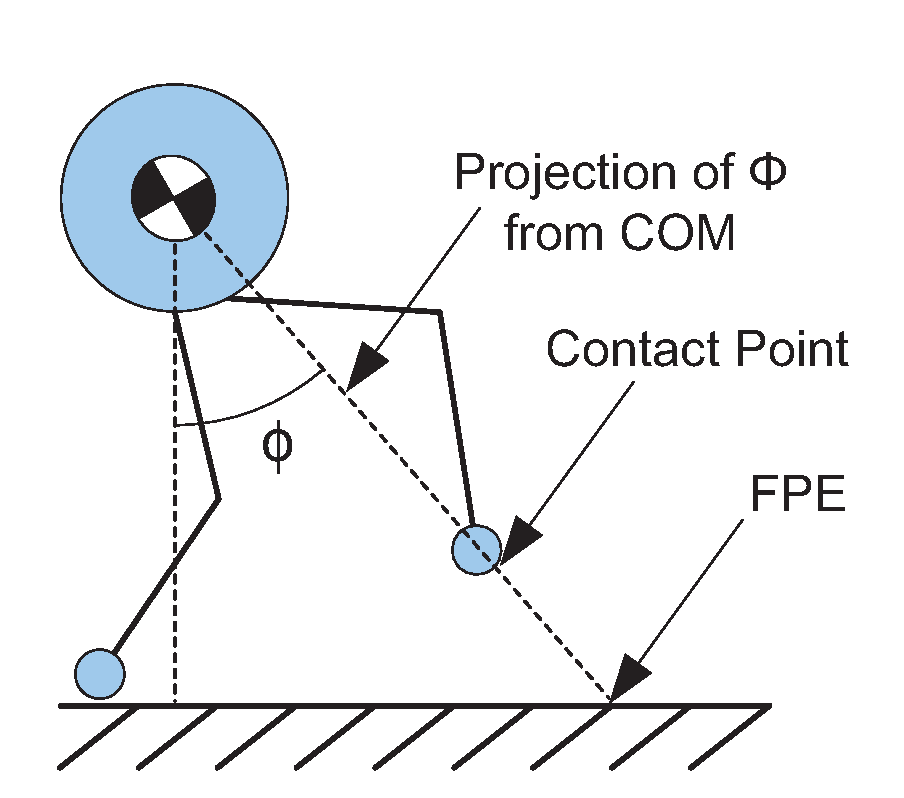
\includegraphics[scale=0.6]{fig/fpe/fig5.eps}
  	\caption{Graphical representation of the solution to the FPE equation for arbitrary robot configurations.}
	\label{fig:phi}
\end{figure}

% subsection computing_the_fpe_angle (end)

\subsection{Stability Analysis} % (fold)
\label{sub:overstepping_understepping_simulation}

In order to show that stepping on the FPE point can restore stability to an unbalanced system, the unified state space model was implemented in simulation along with a numerical solver for the nonlinear FPE equation \eqref{eq:fpe}. Three experiments were devised to analyze the behaviour of the system when the swing foot steps exactly on, behind and ahead of the FPE location obtained from the solver. These three cases are labelled perfect, under and over stepping, respectively. The simulations assume arbitrary physical parameters for $m$, $I_{COM}$, etc. The compass biped model with the single state variable is simulated to illustrate the effects of overstepping and under stepping. The leg separation angle $\beta$ is held constant and no energy is lost upon impact. 

\begin{figure}[!h]
	\begin{center}
	\subfigure{\includegraphics[scale=0.43]{fig/simulations/perfectsteppingtime.eps}}
	\subfigure{\includegraphics[scale=0.43]{fig/simulations/perfectsteppingphase.eps}}
	\end{center}
  	\caption{Time evolution and state trajectories for perfect stepping (i.e. foot lands extactly on the FPE point)}
	\label{sim:perfect}
\end{figure}

The results of the perfect stepping case shown in Figure \ref{sim:perfect} validate the efficacy of the FPE point on the ground. Starting from an unstable configuration, the simple biped model exhibits stability (i.e. rocking back and forth) due to no energy loss in the system by assumption. For a real physical biped, the energy losses experienced during impact would produce a decaying orbit towards the origin due to the asymptotic stability of the system within this local region. 

\begin{figure}[!h]
	\begin{center}
	\subfigure{\includegraphics[scale=0.43]{fig/simulations/understeppingtime.eps}}
	\subfigure{\includegraphics[scale=0.43]{fig/simulations/understeppingphase.eps}}
	\end{center}
  	\caption{Time evolution and state trajectories for under stepping (i.e. foot lands behind FPE point)}
	\label{sim:under}
\end{figure}

In the under stepping case, the swing foot lands short of the FPE location on the ground. This behaviour results in an excessive energy and momentum which causes the biped to eventually fall over. Starting from the same initial conditions presented in the perfect stepping case, the results of understepping is shown in Figure \ref{sim:under}. The time evolution and state trajectories exhibit unstable behaviour, further validating the results presented in \cite{Wight:2008ii}. 

\begin{figure}[!h]
	\begin{center}
	\subfigure{\includegraphics[scale=0.43]{fig/simulations/oversteppingtime.eps}}
	\subfigure{\includegraphics[scale=0.43]{fig/simulations/oversteppingphase.eps}}
	\end{center}
  	\caption{Time evolution and state trajectories for over stepping (i.e. foot lands in front of FPE point)}
	\label{sim:over}
\end{figure}

Lastly, the results of overstepping with the same initial conditions is presented in Figure \ref{sim:over}. As expected, if the swing foot lands ahead of the FPE location, the system enters a stable orbit where the biped rocks back and forth. As mentioned previously, the energy losses experienced during impact for a real biped would cause this closed orbit to decay and eventually reach the equilibrium due to local asymptotic stability. 

% subsection overstepping_understepping_simulation (end)

\subsection{Forming Complete Gait Cycles} % (fold)
\label{sub:gait_cycles}
Wight used the FPE concept to develop full gait cycles using simple linear control techniques and a state machine \cite{Wight:2008vt}. Gait is initiated by destabilizing the robot in the desired direction of movement (forward or backward). Once destabilized, the FPE equation is solved numerically to obtain the FPE angle $\phi$, which is used to provide the desired trajectory for the swing foot. 

\begin{figure}[!h]
	\centering
    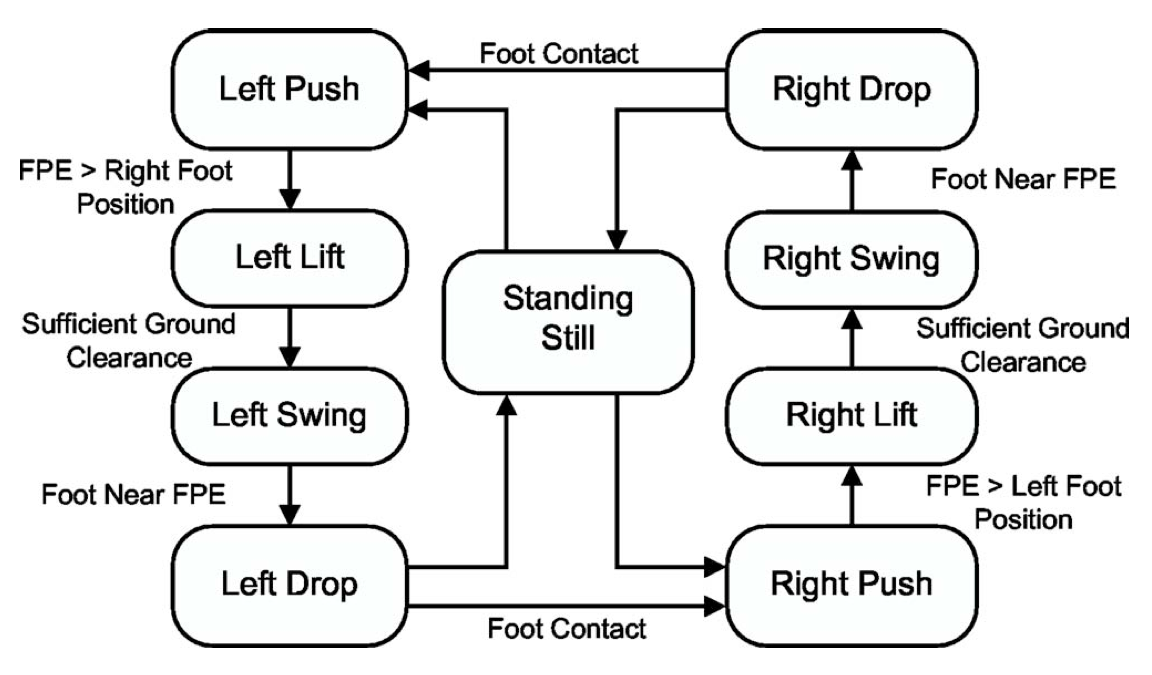
\includegraphics[scale=0.4]{fig/simulations/fpestatemachine.png}
  	\caption{A simple state machine used in conjunction with the FPE algorithm to form complete gait cycles}.
	\label{fig:statemachine}
\end{figure}

If continued forward progress is desired, the foot is commanded to precede the FPE. If no further forward progress is needed, the foot is commanded to the FPE. The desired trajectory is resolved to joint angles using inverse kinematics and implemented via joint level PD controllers. The complete state machine is shown in Figure~\ref{fig:statemachine}. Due to symmetry, the states in Figure~\ref{fig:statemachine} can be reduced to \textbf{STAND}, \textbf{PUSH}, \textbf{LIFT}, \textbf{SWING} and \textbf{DROP}. For the remainder of this paper, the sequence of state transitions from \textbf{PUSH} to \textbf{DROP} is referred to as the step cycle.
% subsection forming_complete_gait_cycles (end)


% section fpe_2D (end)
% chapter background (end) ====================================================